\section{GUI Design}

The FANS web application interface acts as a means for the user to keep track of any potential fires in their
environment. While subject to change, the current interface will look like Figure \ref{fig:homepage} given below. The
interactions between the user and the UI will be explained in detail in the paragraphs below.

\begin{figure}[H]
    \centering
    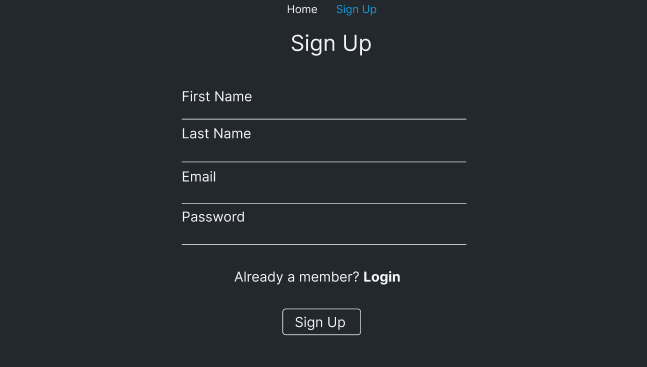
\includegraphics[width=4in]{../assets/gui/SignUpPage.png}
    \caption{GUI mockup for the sign up page of the FANS web app.}
    \label{fig:signup}
\end{figure}

\begin{figure}[H]
    \centering
    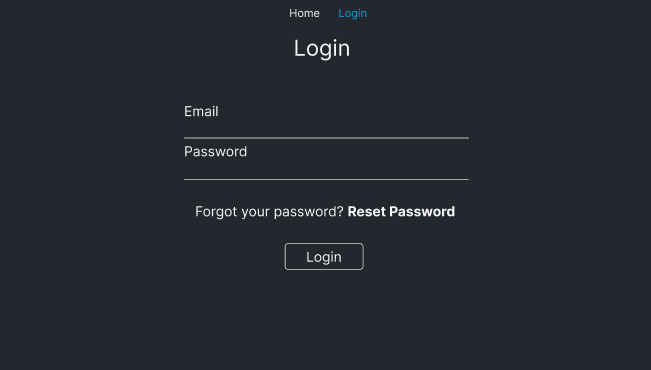
\includegraphics[width=4in]{../assets/gui/LoginPage.png}
    \caption{GUI mockup for the login page of the FANS web app.}
    \label{fig:login}
\end{figure}

The web application is a multi-page dashboard giving the user graphical displays of varying telemetry data gotten from
the fire alarm and notification system. Before gaining access to the home page, the user will be taken to a screen
wherein they can sign up or login. The ability to reset one's password will also be available. Upon authentication, the
user will be able to see their fire alarm and its information. If time permits, the team will add a feature wherein the
user can register multiple fire alarms and monitor their activity concurrently.

\begin{figure}[H]
    \centering
    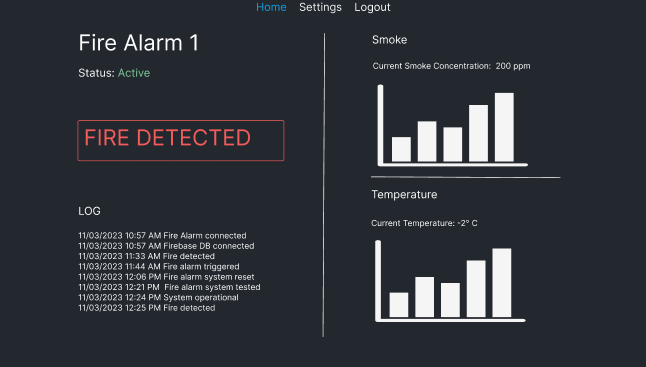
\includegraphics[width=4in]{../assets/gui/HomePage.png}
    \caption{GUI mockup for the home page of the FANS web app.}
    \label{fig:homepage}
\end{figure}

\begin{figure}[H]
    \centering
    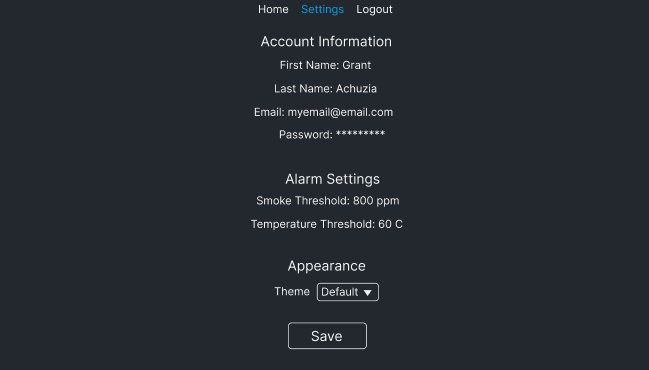
\includegraphics[width=4in]{../assets/gui/SettingsPage.png}
    \caption{GUI mockup for the settings selection page of the FANS web app.}
    \label{fig:settings}
\end{figure}

From the dashboard, the user is able to select a fire alarm and see all the data for the device. Information on the
fire alarm status, smoke detection, surrounding temperature, and fire alarm activity (represented under the LOG in
Figure \ref{fig:login}). The user can also change the detection settings for the fire alarm by navigating to the
settings page.

On the settings page shown in Figure \ref{fig:settings}, the user can view and update their account information, change
the smoke and temperature thresholds (determines when the alarm rings), and choose a theme for the website.

The web application can send notifications from the notification system to an accessory device. When a fire alarm
rings, the status of the UI updates and also changes the status on the accessory device. This device also has the
ability to silence the fire alarm (updating the web applications UI with the new silenced status).

\subsection{Table of Users/Roles}

FANS is designed for two primary users:

\textbf{Building Administrators:} \\
Building administrators will have access to manage the system through the GUI. They have unencumbered access to
configuration changes and can disable the system. These administrators do not necessarily need to be administrators of
larger-scale buildings (office building, etc.) but can also be homeowners.

\textbf{Building Occupants:} \\
Building occupants will be subscribed to the emergency notification alerts by the building administrator, and will
receive updates via email and SMS when an emergency occurs. Those with haptic alarm wearables will also receive a buzz
during an active emergency.
